% 请确保文件编码为utf-8,使用XeLaTex进行编译,或者通过overleaf进行编译

\documentclass[answers]{exam}  % 使用此行带有作答模块
% \documentclass{exam} % 使用此行只显示题目

\usepackage{xeCJK}
\usepackage{zhnumber}
\usepackage{graphicx}
\usepackage{hyperref}
\usepackage{amsmath}
\usepackage{booktabs}
\usepackage{enumerate}

\pagestyle{headandfoot}
\firstpageheadrule
\firstpageheader{南京大学}{数字信号处理}{习题集四}
\runningheader{南京大学}
{数字信号处理}
{习题集四}
\runningheadrule
\firstpagefooter{}{第\thepage\ 页(共\numpages 页)}{}
\runningfooter{}{第\thepage\ 页(共\numpages 页)}{}

% no box for solutions
% \unframedsolutions

\setlength\linefillheight{.5in}

% \renewcommand{\solutiontitle}{\noindent\textbf{答:}}
\renewcommand{\solutiontitle}{\noindent\textbf{解:}\par\noindent}

\renewcommand{\thequestion}{\zhnum{question}}
\renewcommand{\questionlabel}{\thequestion .}
\renewcommand{\thepartno}{\arabic{partno}}
\renewcommand{\partlabel}{\thepartno .}

\begin{document}
\Large
\centering{姓名:左之睿 \qquad  学号:191300087 \qquad 邮箱:1710670843@qq.com}
\begin{questions}
	
	

% question_1
\question 求图~\ref{Figure:question_1}所示各信号的拉普拉斯变换。
\begin{figure}[!h]
	\centering
	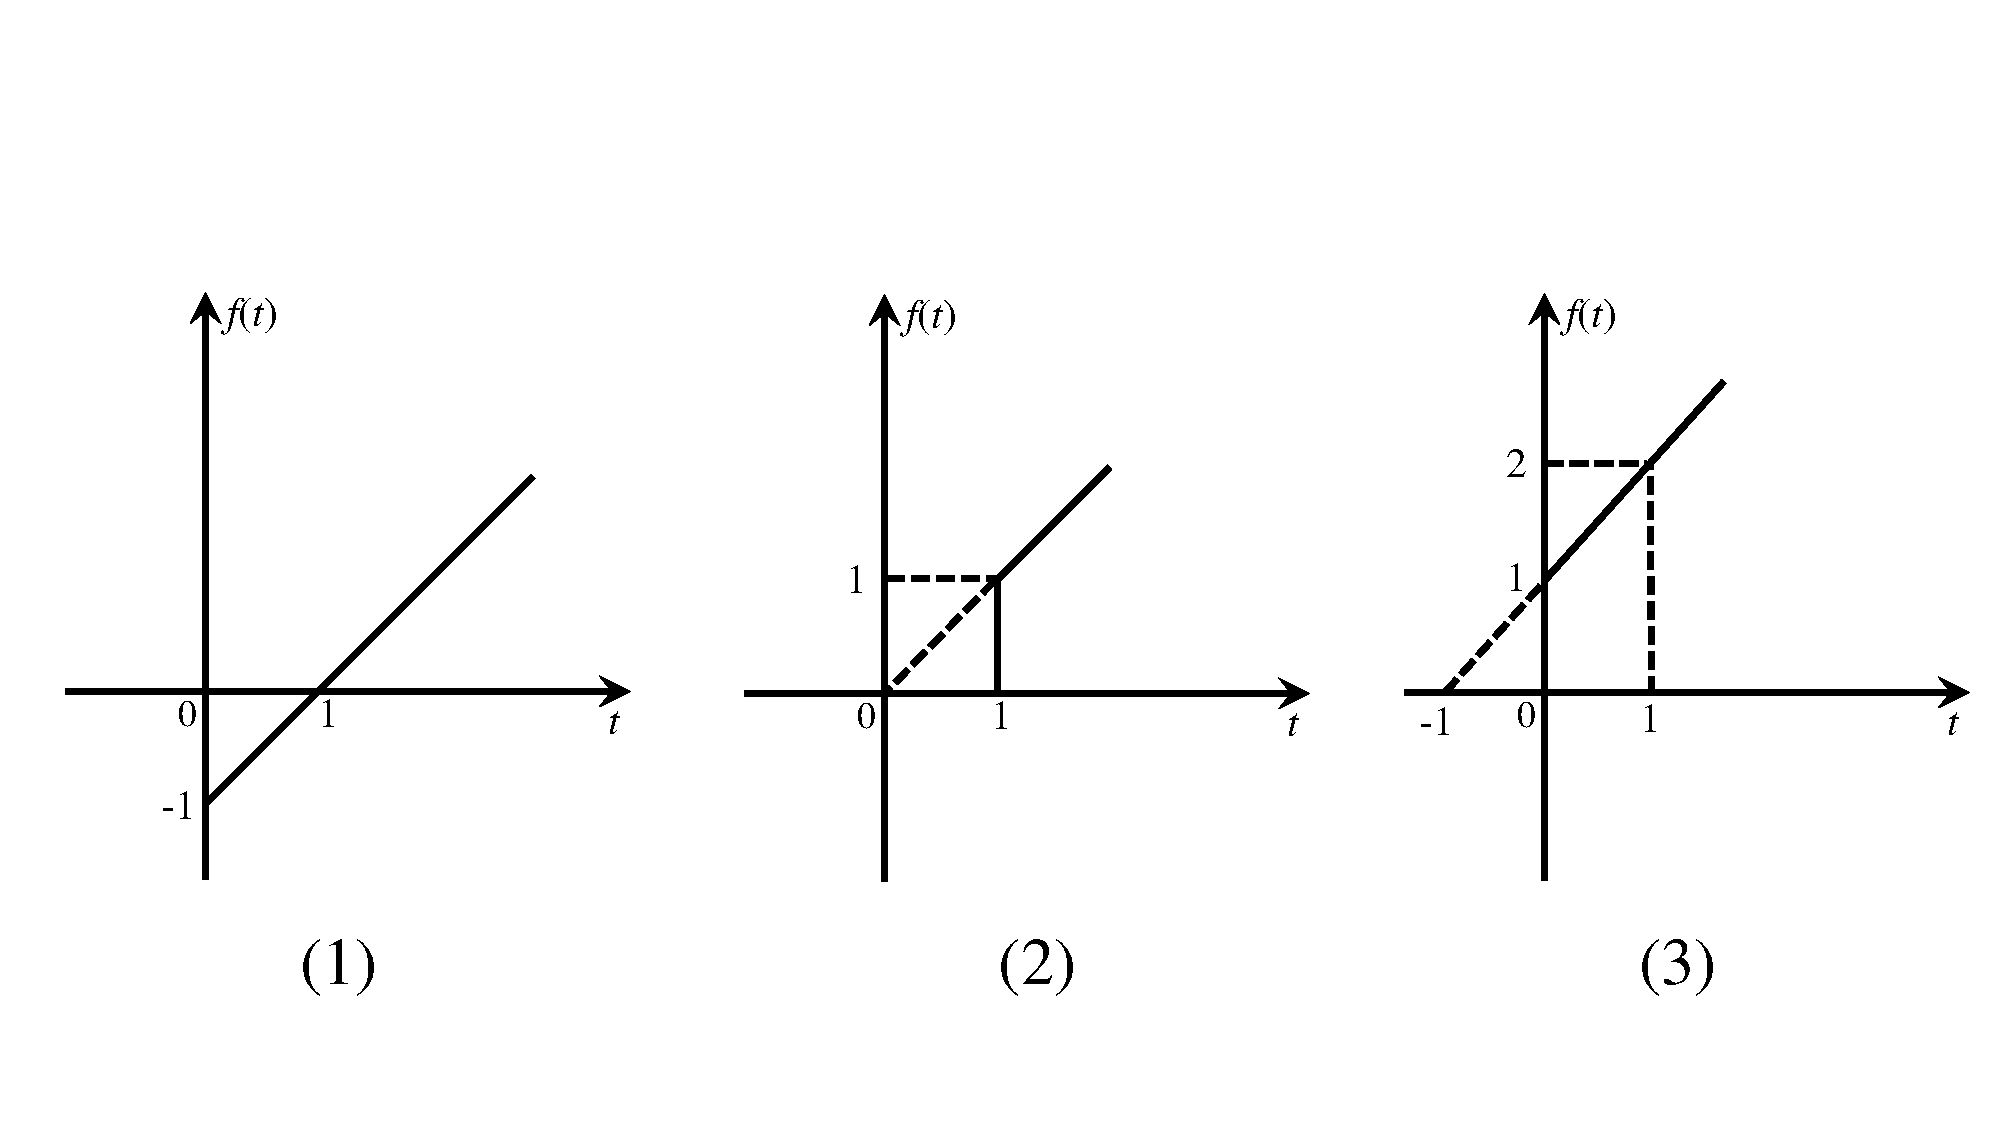
\includegraphics[width=\linewidth]{pics/question_1.pdf}
	\label{Figure:question_1}
	\caption{第一题图}
\end{figure}
\begin{solution}
	(1)、
\begin{align*}
	X(s)&=\int_{0^-}^{\infty}x(t)e^{-st}dt\\
	&=\int_{0^-}^{\infty}(t-1)e^{-st}dt\\
	&=-\frac{1}{s}\int_{0^-}^\infty(t-1)de^{-st}\\
	&=-\frac{1}{s}[(t-1)e^{-st}|_{0^-}^\infty-\int_{0^-}^\infty e^{-st}d(t-1)]\\
	&=-\frac{1}{s}+\frac{1}{s^2}
\end{align*}\\
	~\\
	(2)、
	\begin{align*}
		X(s)&=\int_{1}^{\infty}x(t)e^{-st}dt\\
		&=\int_{1}^{\infty}te^{-st}dt\\
		&=-\frac{1}{s}\int_{1}^{\infty}tde^{-st}\\
		&=-\frac{1}{s}[te^{-st}|_1^{\infty}-\int_{1}^\infty e^{-st}dt]\\
		&=\frac{1}{se^s}+\frac{1}{s^2e^s}
	\end{align*}\\
	~\\
	(3)、	
	\begin{align*}
		X(s)&=\int_{0^-}^{\infty}x(t)e^{-st}dt\\
		&=\int_{0^-}^{\infty}(t+1)e^{-st}dt\\
		&=-\frac{1}{s}\int_{0^-}^\infty(t+1)de^{-st}\\
		&=-\frac{1}{s}[(t+1)e^{-st}|_{0^-}^\infty-\int_{0^-}^\infty e^{-st}d(t+1)]\\
		&=\frac{1}{s}+\frac{1}{s^2}
	\end{align*}
\end{solution}
\newpage
% question_2
\question 求图~\ref{Figure:question_2}所示信号$f(t)$的拉普拉斯变化$F(s)$.
\begin{figure}[!h]
	\centering
	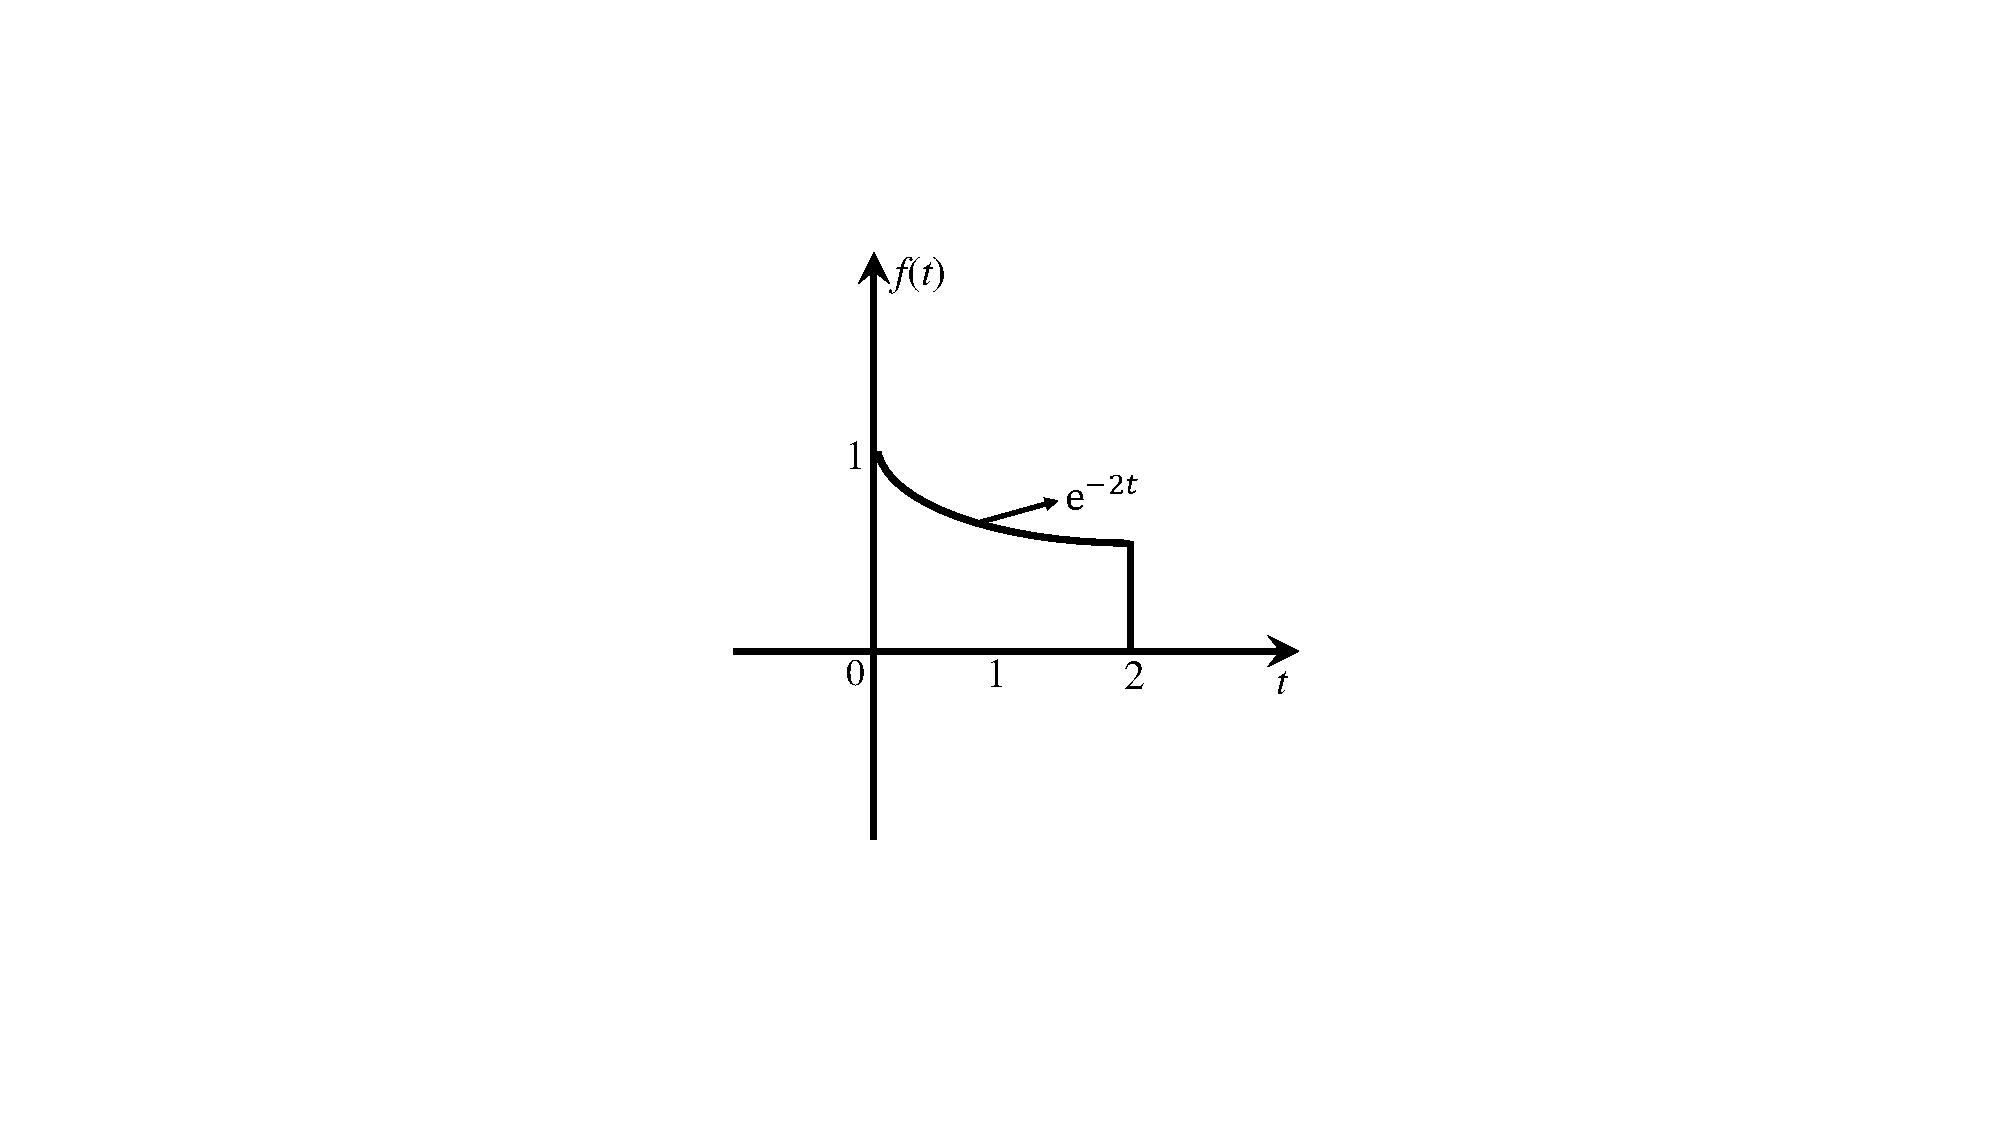
\includegraphics[width=0.3\linewidth]{pics/question_2.pdf}
	\label{Figure:question_2}
	\caption{第二题图}
\end{figure}
\begin{solution}
	\begin{align*}
		F(s)&=\int_{0^-}^\infty f(t)e^{-st}dt\\
		&=\int_0^2 e^{-2t}e^{-st}dt\\
		&=\frac{1-e^{-4-2s}}{s+2}
	\end{align*}
\end{solution}
\newpage
% question_3
\question 某系统函数$H(s)=\frac{1}{s^2+3s+1}$,若输入$x(t)=u(t)$,求出系统的零状态响应$y(t)$。
\begin{solution}
系统的零状态响应$Y(s)=H(s)X(s)=\frac{1}{s(s^2+3s+1)}$\\
对$Y(s)$作分式展开有$$Y(s)=\frac{k_1}{s}+\frac{k_2}{s-(-1.5+0.5\sqrt{5})}+\frac{k_3}{s-(-1.5-0.5\sqrt{5})}$$
$k_1=sY(s)|_{s=0}=1$\\
$k_2=(s-(-1.5+0.5\sqrt{5}))Y(s)|_{s=-1.5+0.5\sqrt{5}}=-\frac{5+3\sqrt{5}}{10}$\\
$k_3=(s-(-1.5-0.5\sqrt{5}))Y(s)|_{s=-1.5-0.5\sqrt{5}}=\frac{3\sqrt{5}-5}{10}$\\
故$$Y(s)=\frac{1}{s}-\frac{\frac{3\sqrt{5}+5}{10}}{s-(-1.5+0.5\sqrt{5})}+\frac{\frac{3\sqrt{5}-5}{10}}{s-(-1.5-0.5\sqrt{5})}$$
所以零状态响应$$y(t)=u(t)-\frac{3\sqrt{5}+5}{10}e^{(-1.5+0.5\sqrt{5})t}u(t)+\frac{3\sqrt{5}-5}{10}e^{(-1.5-0.5\sqrt{5})t}u(t)$$
\end{solution}
\newpage
% question_4
\question 已知某线性时不变系统的微分方程为$\frac{\mathrm{d}^2y(t)}{\mathrm{d}t^2}+4\frac{\mathrm{d}y(t)}{\mathrm{d}t}+3y(t)=2x(t)$。
\begin{enumerate}[(1)]
\item 求该系统的系统函数,画出零极点图并判断该系统是否稳定。
\item 求该系统的冲激响应.
\end{enumerate}
\begin{solution}
(1)、对微分方程两边作拉普拉斯变换,有$$s^2Y(s)-sy(0^-)-y'(0^-)+4[sY(s)-y(0^-)]+3Y(s)=2X(s)$$
求系统函数时,$y(0^-)=0,y'(0^-)=0$,故
$$(s^2+4s+3)Y(s)=2X(s)$$
$$\Downarrow$$
$$H(s)=\frac{Y(s)}{X(s)}=\frac{2}{s^2+4s+3}$$
系统极点$s_1=-1,s_2=-3$均位于s平面的左半部分,故系统稳定,零极点图如下
~\\
(2)、冲激响应$h(t)=\mathcal{L}^{-1}[H(s)]$\\
做部分分式分解$$H(s)=\frac{1}{s+1}-\frac{1}{s+3}$$
所以$$h(t)=e^{-t}u(t)-e^{-3t}u(t)$$
\end{solution}
\begin{figure}[h]
	\centering
	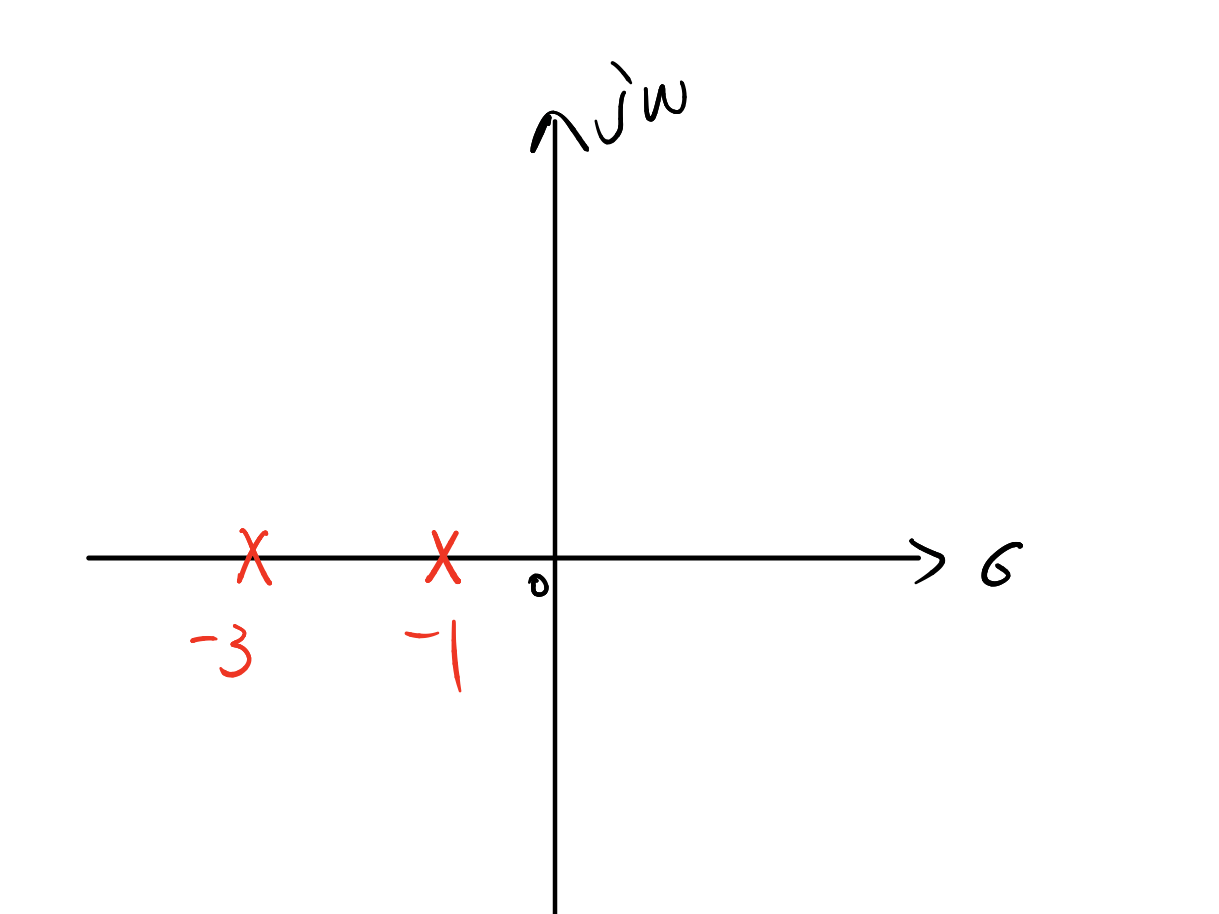
\includegraphics[width=0.3\linewidth]{pics/p4-1.PNG}
	\caption{零极点图}
\end{figure}
\newpage
% question_5
\question 求下列函数的拉普拉斯变换。
\begin{enumerate}[(1)]
\item $f(t)=\left\{\begin{matrix}
\sin(\omega t) & \text{当}\left(0<t<\frac{T}{2} \right )\\ 
 0& t\text{为其他值}
\end{matrix}\right.$

$T=\frac{2\pi}{\omega}$
\item $f(t)=\sin(\omega t+\phi)$
\end{enumerate}
\begin{solution}
(1)、
\begin{align*}
	F(s)&=\int_{0^-}^\infty f(t)e^{-st}dt\\
	&=\int_0^{\frac{T}{2}}sinwt\cdot e^{-st}dt\\
	&=-\frac{w^2}{s^2+w^2}(\frac{1}{w}e^{-st}coswt+\frac{s}{w^2}e^{-st}sinwt)|_0^{\frac{T}{2}}\\
	&=\frac{w}{s^2+w^2}(1+e^{-\frac{sT}{2}})
\end{align*}\\
~\\
(2)、$f(t)=sinwtcos\phi+coswtsin\phi$,故
\begin{align*}
	F(s)&=cos\phi\mathcal{L}[sinwt]+sin\phi\mathcal{L}[coswt]\\
	&=\frac{w\cdot\cos\phi+s\cdot\sin\phi}{s^2+w^2}
\end{align*}
\end{solution}
\newpage
% question_6
\question 求下列函数的拉普拉斯变换。
\begin{enumerate}[(1)]
\item $f(t)=\mathrm{e}^{-t}u(t-2)$
\item $f(t)=\mathrm{e}^{-(t-2)}u(t-2)$
\item $f(t)=\mathrm{e}^{-(t-2)}u(t)$
\item $f(t)=\sin(2t)\cdot u(t-1)$
\item $f(t)=(t-1)[u(t-1)-u(t-2)]$
\end{enumerate}
\begin{solution}
(1)、
\begin{align*}
	F(s)&=\int_{0^-}^\infty f(t)e^{-st}dt\\
	&=\int_2^\infty e^{-t}e^{-st}dt\\
	&=\frac{e^{-2(s+1)}}{s+1},\sigma>-1
\end{align*}
~\\
(2)、
\begin{align*}
	F(s)&=\int_{0^-}^\infty f(t)e^{-st}dt\\
	&=\int_2^\infty e^{-(t-2)}e^{-st}dt\\
	&=\frac{e^{-2s}}{s+1},\sigma>-1
\end{align*}
~\\
(3)、
\begin{align*}
	F(s)&=\int_{0^-}^\infty f(t)e^{-st}dt\\
	&=\int_0^\infty e^{-(t-2)}e^{-st}dt\\
	&=\frac{e^2}{s+1},\sigma>-1
\end{align*}
~\\
(4)、
\begin{align*}
	F(s)&=\int_{0^-}^\infty f(t)e^{-st}dt\\
	&=\int_1^\infty sin(2t)e^{-st}dt\\
	&=\frac{4}{4-s^2}(-\frac{1}{2}e^{-st}cos2t+\frac{s}{4}e^{-st}sin2t)|_1^\infty\\
	&=\frac{2cos2+s\cdot\sin2}{s+4}e^{-s}
\end{align*}
~\\
(5)、
\begin{align*}
	F(s)&=\int_{0^-}^\infty f(t)e^{-st}dt\\
	&=\int_1^2(t-1)e^{-st}dt\\
	&=-\frac{1}{s}(t-1)e^{-st}|_1^2-\frac{1}{s^2}e^{-st}|_1^2\\
	&=-\frac{1}{s}e^{-2s}-\frac{1}{s^2}e^{-2s}+\frac{1}{s^2}e^{-s}
\end{align*}
\end{solution}
\newpage
% question_7
\question 求下列函数的拉普拉斯逆变换。
\begin{enumerate}[(1)]
\item $\frac{1}{s+1}$
\item $\frac{4}{2s+3}$
\item $\frac{4}{s(2s+3)}$
\item $\frac{3}{(s+4)(s+2)}$
\item $\frac{1}{s^2-3s+2}$
\item $\frac{1}{(s^2+3)^2}$
\end{enumerate}
\begin{solution}
(1)、
$$f(t)=\mathcal{L}^{-1}[F(s)]=e^{-t}u(t)$$
~\\
(2)、
$F(s)=2\frac{1}{s+1.5}$,故$$f(t)=2e^{-1.5t}u(t)$$
~\\
(3)、
作分式分解$F(s)=\frac{k_1}{s}+\frac{k_2}{2s+3}$,故\\
$k_1=sF(s)|_{s=0}=\frac{4}{3}$\\
$k_2=(2s+3)F(s)|_{s=-1.5}=-\frac{8}{3}$\\
即$$F(s)=\frac{4}{3}\cdot\frac{1}{s}-\frac{8}{3}\frac{1}{2s+3}$$
所以$$f(t)=\frac{4}{3}u(t)-\frac{4}{3}e^{-1.5t}u(t)$$
~\\
(4)、
作分式分解$F(s)=\frac{k_1}{s+4}+\frac{k_2}{s+2}$,故\\
$k_1=(s+4)F(s)|_{s=-4}=-1.5$\\
$k_2=(s+2)F(s)|_{s=-2}=1.5$\\
即$$F(s)=-1.5\frac{1}{s+4}+1.5\frac{1}{s+2}$$
所以$$f(t)=-1.5e^{-4t}u(t)+1.5e^{-2t}u(t)$$
~\\
(5)、$F(s)=\frac{1}{s^2-3s+2}=\frac{1}{(s-1)(s-2)}$\\
作分式分解$F(s)=\frac{1}{s-2}-\frac{1}{s-1}$\\
所以$$f(t)=-e^tu(t)+e^{2t}u(t)$$
~\\
(6)、考虑到$\mathcal{L}[sin\sqrt{3}t]=\frac{\sqrt{3}}{s^2+3}$\\
故计算$f(t)=tsin\sqrt{3}t$的laplace变换\\
\begin{align*}
	F(s)&=\int_{0^-}^\infty tsin\sqrt{3}t\cdot e^{-st}dt\\
	&=-\frac{1}{\sqrt{3}}\int_{0^-}^\infty te^{-st}dcos\sqrt{3}t\\
	&=-\frac{1}{\sqrt{3}}[te^{-st}cos\sqrt{3}t|_{0^-}^\infty-\int_{0^-}^\infty cos\sqrt{3}td(te^{-st})]\\
	&=\frac{1}{\sqrt{3}}\int_{0^-}^\infty e^{-st}cos\sqrt{3}tdt-\frac{s}{\sqrt{3}}\int_{0^-}^\infty te^{-st}cos\sqrt{3}tdt\\
	&=\frac{1}{\sqrt{3}}\mathcal{L}[cos\sqrt{3}t]+\frac{s}{3}\int_{0^-}^\infty sin\sqrt{3}td(te^{-st})\\
	&=\frac{1}{\sqrt{3}}\mathcal{L}[cos\sqrt{3}t]+\frac{s}{3}\mathcal{L}[sin\sqrt{3}t]-\frac{s^2}{3}F(s)
\end{align*}
故$$F(s)=\frac{3}{3+s^2}(\frac{1}{\sqrt{3}}\cdot\frac{s}{s^2+3}+\frac{s}{3}\cdot\frac{\sqrt{3}}{s^2+3})=\frac{2\sqrt{3}s}{(s^2+3)^2}$$
由积分性质和线性性$$\mathcal{L}[\frac{1}{2\sqrt{3}}\int f(t)dt]=\frac{1}{(s^2+3)^2}$$
~\\
所以最终求得的拉普拉斯逆变换为:
\begin{align*}
	&\frac{1}{2\sqrt{3}}\int tsin\sqrt{3}tdt\\
	=&\frac{1}{2\sqrt{3}}(-\frac{1}{\sqrt{3}}tcos\sqrt{3}t+\frac{1}{\sqrt{3}}\int cos\sqrt{3}tdt)\\
	=&-\frac{t}{6}cos\sqrt{3}t+\frac{1}{6\sqrt{3}}sin\sqrt{3}t
\end{align*}
\end{solution}
\newpage
% question_8
\question 离散系统的差分方程为$y[n]-2y[n-1]=x[n]$,激励$x[n]=3^{n}u[n],y[0]=2$,求响应$y[n]$。
\begin{solution}
	对差分方程两边做Z变换,有$$Y(z)-2z^{-1}Y[z]-2y[-1]=X(z)$$
	由差分方程$y[0]-2y[-1]=x[0]\rightarrow y[-1]=0.5$\\
	而$X(z)=\sum_{i=0}^{\infty}3^{i}z^{-i}=\frac{1}{1-3z^{-1}}$
	所以差分方程为$$(1-2z^{-1})Y(z)-1=\frac{1}{1-3z^{-1}}$$
	$$\Downarrow$$
	$$Y(z)=\frac{2-3z^{-1}}{(1-3z^{-1})(1-2z^{-1})}$$
	做部分分式分解,有$Y(z)=\frac{3}{1-3z^{-1}}-\frac{1}{1-2z^{-1}}$\\
	故$$y[n]=3^{n+1}u[n]-2^nu[n]$$
\end{solution}
\newpage
% question_9
\question 已知离散时间单位阶跃信号$u[n]$的$z$变换为$\frac{1}{1-z^{-1}},|z|>1$,利用$z$变换的性质求信号$n^2u[n]$的$z$变换。
\begin{solution}
	先使用一次z域微分特性$${\mathcal{Z}}[nu[n]]=X_1(z)=-z\frac{dX(z)}{dz}=\frac{z^{-1}}{(1-z^{-1})^2}$$
	再使用一次z域微分特性$$\mathcal{Z}[n\cdot nu[n]]=-z\frac{dX_1(z)}{dz}=\frac{z^{-1}(1+z^{-1})}{(1-z^{-1})^3}$$
\end{solution}
\newpage
% question_10
\question 求下列$X(z)$的逆变换$x[n]$。
\begin{enumerate}[(1)]
\item $X(z)=\frac{10}{(1-0.5z^{-1})(1-0.25z^{-1})},(|z|>0.5)$
\item $X(z)=\frac{10z^2}{(z-1)(z+1)},(|z|>1)$
\end{enumerate}
\begin{solution}
	(1)、作部分分式分解$X(z)=\frac{20}{1-0.5z^{-1}}-\frac{10}{1-0.25z^{-1}}$\\
	故$$x[n]=20\cdot(0.5)^nu[n]-10\cdot(0.25)^nu[n]$$
	~\\
	(2)、$X(z)=\frac{10}{(1+z^{-1})(1-z^{-1})}$\\
	做部分分式分解$X(z)=\frac{5}{1+z^{-1}}+\frac{5}{1-z^{-1}}$\\
	故$$x[n]=5u[n]+5(-1)^nu[n]$$
\end{solution}
\newpage
% question_11
\question 用单边$z$变换解下列差分方程。
\begin{enumerate}[(1)]
\item $y[n+2]+y[n+1]+y[n]=u[n],y[0)]=1,y[1]=2$
\item $y[n]+0.1y[n-1]-0.02y[n-2]=10u[n],y[-1]=4,y[-2]=6$
\item $y[n]=-5y[n-1]+nu[n],y[-1]=0$
\end{enumerate}
\begin{solution}
	(1)、对差分方程两边做Z变换\\
	$$(z^2Y(z)-z^2y[0]-zy[1])+(zY(z)-zy[0])+Y(z)=\frac{1}{1-z^{-1}}$$
	$$\Downarrow$$
	$$Y(z)=\frac{-2z^{-2}+2z^{-1}+1}{(1-z^{-1})(z^{-2}+z^{-1}+1)}$$
	做部分分式分解
	$$Y(z)=\frac{1}{3}\cdot\frac{1}{1-z^{-1}}+\frac{\frac{7}{3}z^{-1}+\frac{2}{3}}{z^{-2}+z^{-1}+1}$$
	其中,第2项可以改写成$$\frac{\frac{2}{3}(1-z^{-1}cos\frac{2\pi}{3})}{z^{-2}-2z^{-1}cos(\frac{2\pi}{3})+1}+\frac{\frac{4}{\sqrt{3}}z^{-1}sin\frac{2\pi}{3}}{z^{-2}-2z^{-1}cos(\frac{2\pi}{3})+1}$$
	再做Z反变换,得到
	$$y[n]=\frac{1}{3}u[n]+\frac{2}{3}cos(\frac{2\pi}{3}n)u[n]+\frac{4}{\sqrt{3}}sin(\frac{2\pi}{3}n)u[n]$$
	~\\
	(2)、对差分方程两边做Z变换\\
	$$Y(z)+0.1(z^{-1}Y(z)+y[-1])-0.02(z^{-2}Y(z)+z^{-1}y[-1]+y[-2])=\frac{10}{1-z^{-1}}$$
	$$\Downarrow$$
	$$Y(z)=\frac{4z^{-2}-18z^{-1}-486}{(1-z^{-1})(z^{-1}+5)(z^{-1}-10)}$$
	做部分分式分解
	$$Y(z)=9.26\cdot\frac{1}{1-z^{-1}}+0.66\cdot\frac{1}{1+0.2z^{-1}}-0.2\cdot\frac{1}{1-0.1z^{-1}}$$
	$$\Downarrow$$
	$$y[n]=9.26u[n]+0.66(-0.2)^nu[n]-0.2(0.1)^nu[n]$$
~\\
	(3)、对差分方程两边做Z变换$Y(z)=-5(z^{-1}Y(z)+y[-1])+\frac{z^{-1}}{(1-z^{-1})^2}$\\
	由差分方程$y[0]=-5y[-1]\rightarrow y[0]=0$\\
		故$$Y(z)+5z^{-1}Y(z)=\frac{z^{-1}}{(1-z^{-1})^2}$$
	$$\Downarrow$$
	$$Y(z)=\frac{z^{-1}}{(1+5z^{-1})(1-z^{-1})^2}$$
	做部分分式分解$$Y(z)=-\frac{5}{36}\cdot\frac{1}{1+5z^{-1}}+\frac{1}{36}\cdot\frac{1}{1-z^{-1}}+\frac{1}{6}\cdot\frac{1}{(1-z^{-1})^2}$$
	$$\Downarrow$$
	$$y[n]=-\frac{5}{36}\cdot(-5)^nu[n]-\frac{1}{36}\cdot u[n]+\frac{1}{6}\cdot(n+1)u[n]$$
	$$\Downarrow$$
	$$y[n]=\frac{5}{36}\cdot u[n]+\frac{n}{6}u[n]-\frac{5}{36}\cdot(-5)^nu[n]$$
\end{solution}
\newpage
% question 12
\question (选做)你对这门课程的建议。
\begin{solution}
	书面作业量有点少,可以稍微多加一些量便于课后巩固。\\
	编程题很有启发性,挑战性很强,希望下一届可以继续保持出题的水准(我认为难度还可以再往上提一提),进一步考察同学们对傅里叶变换,f-principle等知识的理解与应用。
\end{solution}


\end{questions}
\end{document}